% This is "sig-alternate.tex" V2.0 May 2012
% This file should be compiled with V2.5 of "sig-alternate.cls" May 2012
%
% This example file demonstrates the use of the 'sig-alternate.cls'
% V2.5 LaTeX2e document class file. It is for those submitting
% articles to ACM Conference Proceedings WHO DO NOT WISH TO
% STRICTLY ADHERE TO THE SIGS (PUBS-BOARD-ENDORSED) STYLE.
% The 'sig-alternate.cls' file will produce a similar-looking,
% albeit, 'tighter' paper resulting in, invariably, fewer pages.
%
% ----------------------------------------------------------------------------------------------------------------
% This .tex file (and associated .cls V2.5) produces:
%       1) The Permission Statement
%       2) The Conference (location) Info information
%       3) The Copyright Line with ACM data
%       4) NO page numbers
%
% as against the acm_proc_article-sp.cls file which
% DOES NOT produce 1) thru' 3) above.
%
% Using 'sig-alternate.cls' you have control, however, from within
% the source .tex file, over both the CopyrightYear
% (defaulted to 200X) and the ACM Copyright Data
% (defaulted to X-XXXXX-XX-X/XX/XX).
% e.g.
%% \CopyrightYear{2016} will cause 2007 to appear in the copyright line.
% \crdata{0-12345-67-8/90/12} will cause 0-12345-67-8/90/12 to appear in the copyright line.
%
% ---------------------------------------------------------------------------------------------------------------
% This .tex source is an example which *does* use
% the .bib file (from which the .bbl file % is produced).
% REMEMBER HOWEVER: After having produced the .bbl file,
% and prior to final submission, you *NEED* to 'insert'
% your .bbl file into your source .tex file so as to provide
% ONE 'self-contained' source file.
%
% ================= IF YOU HAVE QUESTIONS =======================
% Questions regarding the SIGS styles, SIGS policies and
% procedures, Conferences etc. should be sent to
% Adrienne Griscti (griscti@acm.org)
%
% Technical questions _only_ to
% Gerald Murray (murray@hq.acm.org)
% ===============================================================
%
% For tracking purposes - this is V2.0 - May 2012

\documentclass{sig-alternate}

\usepackage{url}

\begin{document}
%
% --- Author Metadata here ---
\conferenceinfo{DATECH}{2016 Pozna\'n, Poland}
%\CopyrightYear{2007} % Allows default copyright year (20XX) to be over-ridden - IF NEED BE.
%\crdata{0-12345-67-8/90/01}  % Allows default copyright data (0-89791-88-6/97/05) to be over-ridden - IF NEED BE.
% --- End of Author Metadata ---

\title{
  Enabling Annotation of Historical Corpora in an Asynchronous Collaborative Environment
    \titlenote{
    This research was supported by ...
  }  
}
%% \subtitle{
  %% [Extended Abstract] Do we need a subtitle?

%% }

%
% You need the command \numberofauthors to handle the 'placement
% and alignment' of the authors beneath the title.
%
% For aesthetic reasons, we recommend 'three authors at a time'
% i.e. three 'name/affiliation blocks' be placed beneath the title.
%
% NOTE: You are NOT restricted in how many 'rows' of
% "name/affiliations" may appear. We just ask that you restrict
% the number of 'columns' to three.
%
% Because of the available 'opening page real-estate'
% we ask you to refrain from putting more than six authors
% (two rows with three columns) beneath the article title.
% More than six makes the first-page appear very cluttered indeed.
%
% Use the \alignauthor commands to handle the names
% and affiliations for an 'aesthetic maximum' of six authors.
% Add names, affiliations, addresses for
% the seventh etc. author(s) as the argument for the
% \additionalauthors command.
% These 'additional authors' will be output/set for you
% without further effort on your part as the last Section in
% the body of your article BEFORE References or any Appendices.

\numberofauthors{2} %  in this sample file, there are a *total*
% of EIGHT authors. SIX appear on the 'first-page' (for formatting
% reasons) and the remaining two appear in the \additionalauthors Section.
%
\author{
% You can go ahead and credit any number of authors here,
% e.g. one 'row of three' or two rows (consisting of one row of three
% and a second row of one, two or three).
%
% The command \alignauthor (no curly braces needed) should
% precede each author name, affiliation/snail-mail address and
% e-mail address. Additionally, tag each line of
% affiliation/address with \affaddr, and tag the
% e-mail address with \email.
%
% 1st. author
\alignauthor
Enrique Manjavacas Ar\'evalo\\
\affaddr{Universiteit Antwerpen}\\
\affaddr{R.112, Rodestraat 14}\\
\affaddr{Antwerp 2000, Belgium}\\
\email{enrique.manjavacas@uantwerpen.be}
% 2nd. author
\alignauthor
Peter Petr\'e\\
\affaddr{Universiteit Antwerpen}\\
\affaddr{R.229, Rodestraat 14}\\
\affaddr{Antwerp 2000, Belgium}\\
\email{peter.petre@uantwerpen.be}
}

\maketitle
\begin{abstract}
  Current research in Corpus Linguistics and other related disciplines within the
  multi-disciplinary field of Digital Humanities, involves computer-aided manual processing
  of large text corpora. Typically, corpus instances are retrieved with the help of
  concordancers and textual search engines and subsequently labeled by hand before being
  submitted to quantitative or qualitative analysis.
  While well-established systems already cover the data retrieval aspect,
  less attention has been paid to the annotation process in terms of both software
  facilities and best practices. However, with the current increase in size and scope
  of research projects we envisage new needs for synchronizing interdependent
  analysis metadata by different researchers.
  Current ad-hoc solutions typically involve general-purpose Real-Time Editing (RTE)
  and cloud storage software, whose functionality are arguably sub-optimal for research purposes.
  In the present paper we will discuss potential problems related to coordinating
  annotations in large-scale projects as well as the potential benefits that can be
  derived from an application-based approach to annotation data management.
  Furthermore, we discuss some of the design choices that have to be taken regarding the
  nature of collaborative software. Finally, we showcase our current implementation of a
  collaborative asynchronous system in the context of a Historical Linguistics research
  project involving several parallel studies and multiple researchers.
\end{abstract}

%% A category with the (minimum) three required fields
%% https://cran.r-project.org/web/classifications/ACM.html
\category{J.5}{Computer Applications}{Arts and Humanities}
\category{I.7.1}{Document and Text Processing}{Document and Text Editing}
%% \category{I.6.5}{Simulation and Modelling}{Model Development}

\keywords{Corpus Annotations, Asynchronous Collaboration, Groupware}

\section{Introduction}\label{sec:intro}
Current corpus-based research practices entail interacting with a single ground-truth
collection of documents \textemdash i.e. a corpus \textemdash, to which analysis metadata
such as annotations are added.

In a context in which the responsibility for the design of the research is not shared
amongst several researchers, decisions as to how to create, design and manage annotation
metadata may be considered unproblematic. However, with the current increase in size and scope of
research projects in Digital Humanities and related fields, we expect new issues to arise from
the need for synchronization of concurrent research activities which could otherwise lead to
inconsistency in the annotation metadata.

Although to our knowledge no prior studies have addressed the issue \textemdash both in terms of
established practices and available tools, %% [TODO: look for (tentative) studies in this direction.]
it can be assumed that a large part of current research requiring support for a
collaborative environment typically resorts to (i) general-purpose Real-Time document Editing
(RTE) software in the best case\footnote{
  See, for instance, \cite{Rowlands2011} and \cite{Wood2011}, for examples of reports on
  using Google Docs for research.
}, (ii) cloud-storage services such as DropBox \cite{Dropboxa}, which provide versioning but do
not support proper collaborative editing of documents\footnote{
  For instance, DropBox explicitly recommends users to modify shared documents outside the scope
  of the synchronization functionality to avoid the creation of conflicting copies \cite{Dropbox}.
}, or (iii) simply avoiding direct collaboration by implementing ad-hoc heuristics \textemdash for
instance, splitting the total annotation load in non-overlapping chunks to be annotated by
single researchers.

%% [TODO: Brief description of the research project]
In any case, inconsistency issues still has to be addressed. In general, inconsistency may arise
for reasons that are both intrinsic and extrinsic to the research activity \textemdash i.e. having
to do, respectively, with interpretational disagreements as to the content and scope of annotations,
and problems related to concurrent modification of the annotation metadata by several researchers.
In particular, we are confronted with the following problems:
\begin{itemize}
\item Unifying label conventions and tagging system, which may not be given as closed
  set tagging system prior to research or may subject to revision renegotiation.
\item Synchronizing the introduction and removal of labels into dynamic tag systems,
  guaranteeing that these updates do not lead to an inconsistent tag system.
\item Ensuring that every involved researcher is notified of parallel work by other members
  of her team, allowing for in-place discussion of issues interfering with their own analyses.
\item Allowing changes to existing annotations to be back-traceable and documented, providing
  a means for resetting to previous versions and for logging the motivations
  that led to the change (in the form of change logs, threaded discussions etc.).
\end{itemize}

Furthermore, a principled solution to collaborative corpus-based research is not only
desirable for the sake of the aforementioned synchronization issues, but it also provides
a number of associated advantages which have the potential to improve the quality of the research.
For instance, managing annotation metadata through a specialized application implies
having available these metadata in a unified and structured shape, easily allowing
for the following features:

\begin{itemize}
\item Easy export and re-formatting functionality.
\item Storage of metadata in a database or indexing through a search engine.
\item Advance querying of the metadata.
\item Visualizing the metadata both as time snapshot and evolution over time.
\item Enable meta-research on research practices thanks to the availability of structured
  metadata derived from the researcher activities (annotation updates, user behavior, etc.).
\end{itemize}

In the present paper we sketch an application-based approach addressing the aforementioned
issues in a way that fits better the concrete needs of the practitioner.
More concretely, we propose to address the problem of managing concurrent annotation
metadata by multiple researchers in the terms of collaborative working systems.
Therefore, in Sections \ref{subsec:rte} and \ref{subsec:vcs}, we will review two major and
not necessarily competing approaches to concurrent multi-user document editing
(Real-time document Editing systems and Version Control Systems).
Next, in Section \ref{subsec:hybrid}, we argue that a hybrid approach may be better suit for
the issues established in the current Section.
In Section \ref{sec:case}, we describe the research infrastructure that we have implemented
following the design principles discussed in Section \ref{sec:cde}.
Finally, in Section \ref{sec:future} we shall highlight lines of further research before
concluding in \ref{sec:conclusion}.

\section{Collaborative Editing}\label{sec:cde}
Collaborative editing refers to the practice by which dispersed
users are able to concurrently modify shared artifacts with the guarantee that changes
by different users will not overwrite each other \textemdash see also \cite{Altmanninger2009}.
Currently, collaborative software has become ubiquitous thanks to Web 2.0 services, such as
Google's web-based suite Google Docs \cite{Googlea} or Microsoft's Office Online \cite{Microsoft}.

We note, however, that other approaches are available beyond the RTE framework. In
particular, Version Control Systems (VCS) \textemdash also known as Revision Control
Systems (RCS), or Concurrent Versioning Systems (CVS) \textemdash, represent a solution
to collaborative editing that is often overlooked due arguably to its less user-friendly
nature and more complex document updates procedures.

In general, RTE and VCS can be seen as alternative solutions to collaborative
editing \cite{Altmanninger2009}, differing with respect to, respectively, whether edit
operations are non-blocking synchronous operations, and immediately reflected on the shared
data, or asynchronous \textemdash i.e. updates are first piped
through a working copy which is only sporadically merged with the source document.
In the next two Sections (\ref{subsec:rte} and \ref{subsec:vcs}) we summarily describe RTE
and VCS systems.

\subsection{Real-Time document Editing}\label{subsec:rte}
RTE software systems aim at solving the synchronous flavor of the collaborative editing
problem, which can be describe in terms of the following two-step procedure \cite{Imine2009}:
first, local changes are immediately reflected in the local copy of the document and, secondly,
the changes are propagated to other users across the network.
More concretely, RTE systems can be defined by the following characteristics \cite{Sun1998}:
(i) the user responsible for a change is able to observe it \textit{real-time};
(ii) collaboration is allowed to take place in a \textit{distributed} way across
different networks \textemdash which involves a layer of non-deterministic communication
latency; (iii) the system allows for \textit{unconstrained}, non-locking edit operations
\textemdash i.e. any user can edit the shared data at any time.

Thus, one major technical puzzle a RTE system has to solve consists of the fact that changes
are propagated across networks with different communication latencies, therefore not
reaching all end-points in the same order. For example, given
the string ``efecte'' and concurrent edit operations \textit{Ins(2, ``f'')} \textemdash i.e.
insert character ``f'' at position 2 \textemdash and \textit{Del(5)} \textemdash i.e.
delete character at position 5: ``e'' \textemdash, the spell-corrected string ``effect''
can only be obtained if \textit{Del(5)} is executed before \textit{Ins(2, ``f'')}.
But if the operations were issued by different users and reached a third user in different
order due to different communication latencies in the network,
the document seen by the third user would reflect an inconsistent state.

A common solution to consistency maintenance is Operational Transformation
(OT) \cite{SuClarence}, a technique that consists in a rule-based transformation
of edit operations which amends the position of an edit operation against a previous edit.
In the previous example, the edit sequence \textit{[Ins(2, ``f''), Del(5)]} should be
transformed as follows:
\begin{equation*}
  \textit{OT([Ins(2, ``f''), Del(5)])} \Rightarrow \textit{[Ins(2, ``f''), Del(6)]}
\end{equation*}
to ensure consistency with respect to the alternative edit sequence
\textit{[Del(5), Ins(2, ``f'')]}.

%% Three types of divergences:
%% Divergence
%% Causality Violation
%% Intention Violation

Finally, OT-based RTE systems work with linear data-structures, typically lists of
characters, but it is possible to work with list of elements at other levels, such as words,
paragraphs or XML nodes \cite{Imine2009,SuClarence}. For instance, in a RTE annotation application,
one might want to consider labels (annotation keys and values) instead of characters as the
atomic targets of edit operations.

%% Limitations...?

\subsection{Version Control System}\label{subsec:vcs}

VCSs have a large tradition originating in the 1970s as groupware for enabling collaborative
software development and more recently have become widely adopted as a result of
integration with a social network environment (GitHub, BitBucket).
Current VCSs follow the copy-modify-merge model, also known as ``optimistic'', to
collaborative document editing, in opposition to the ``pessimistic'' lock-modify-unlock model
in use among early VCSs such as SCCS, RCS or CVS \cite{Loeliger2012}.
In order to guarantee consistency maintenance the lock-modify-model forces users to first
acquire a lock for the target file and release it once changes are finished. However, 
the lock model proved to be too restrictive in practice.

The optimistic flavor of VCS represents an asynchronous collaboration model based on a
two-step procedure of local editing and merging with the shared document.

In principle, this two-step procedure resembles the one described in Section \ref{subsec:rte}
for RTE systems. However, they essentially differ in that in VCS local changes are not merged
immediately (synchronously) into the shared document (as opposed to edit propagation
within the RTE framework); instead they are ``commited'' at a later stage
\textemdash i.e. asynchronously.
By separating edit and merge logic real-time responsiveness is
sacrificed but in exchange two crucial features are gained: (i) the concept of a
\textit{working copy}, (ii) the fact that edits are meaningful \textemdash in the sense
that successful merges can be deemed as intended \textit{versions} of the document.
We now turn to these aspects in more depth.

\subsubsection{Working copy}\label{subsec:workingcopy}
A working copy is a local copy of the shared document that allows users
to modify the document (in their local environment) despite parallel work by other users
\cite{Collins-Sussman}. The concept of working copy has the potential for VCS implementations
that are completely distributed \textemdash known as DVCS (Distributed Version Control Systems).
%citation needed?

The general collaborative workflow with working copies can be described as follows:
When a user wants to update the shared data to reflect the local changes in her working copy
(commits), a ``push'' operation is issued. Similarly, other users can update their local
working copies to reflect the current state of the shared data \textemdash an operation
known as ``pull'' in some implementations of this model.
In both cases a conflict between the local and shared copies may arise if (i) the shared
copy was successfully updated in a particular way by another user before the local changes
are pushed, (ii) or there have been local changes incompatible with the shared copy before
the latter is pulled.
VCS provides a merging mechanism to solve these potential version divergences known as
three-way merging, which involves all three document copies (both conflicting copies and their
shared ancestor) \cite{Altmanninger2009}. In general, VCSs provide automatic merging in cases
of ``syntactically'' unambiguous and it is commonly resorted to manual merging in cases
of ``semantic'' ambiguity, in which conflicting edit intentions may be present.%citation needed.

A crucial aspect of working copies is that they allow for more complex and flexible workflows
than the previously depicted case of a single working copy. In particular, users may create
multiple working copies, each of which can focus on a certain aspect of the project, and
delay merging to a later stage.
By this token, the workflow can be seen as a tree of branches (working copies
representing parallel versions of the shared data) that are being splitted and merged with
the trunk (the shared data)\footnote{
  Strictly speaking, the graph structure resulting from the collaborative model of copy-edit-merge
  with branching does not correspond to a tree due to the presence of merges but rather to a
  Directed Acyclic Graph (DAG).
}.

\subsubsection{Versioning}\label{subsec:versioning}
Versioning is a powerful feature for backtracking changes and restoring project state to a
previous one. Versions can be generally defined as the state of a document in a given time point.
In the context of VCSs, a version refers to the project state resulting from a successful commit.
Moreover, the asynchronous nature of VCS commits allows to attach metadata to changes before
commiting. This is in opposition to RTE document edits that are triggered automatically
after any modification and propagated to other users.

Besides enabling responsibility traceability, version metadata provide grounds to build useful
collaborative features with respect to the following two aspects: (i) edits to a document become
meaningful allowing for the specification of the motivations behind the edit as well as to link
to metadata in previous versions in a structured way \textemdash while structuring of the metadata
is not enforced by default, it can be easily introduced by following particular internal project
conventions; (ii) the resulting tree-shaped edit history can be easily traversed back, choosing
which particular development branch should be followed, and therefore enabling more specific
state restoration.

Finally, as a consequence of the concept of working copies, project state can be again restored
to a certain version independently of concurrent actions by other users, allowing for parallel
versions of the same document. In fact, another popular feature of VCS implementations
is ``forking'' (creating a parallel version of the project, which may eventually be merged
again with the original trunk).

%% \begin{verbatim}
%%   {"word": "the", "pos": "AT"} \\ Brown Tagset
%%   {"word": "the", "pos": "DT"} \\ PTB Tagset
%% \end{verbatim}

%%                      _branch: brown->PTB     _ merge
%%                     /                         \
%% - user1 uses brown - continue adding more PTB  --
%%                                                   - merge ----
%% - user2 uses PTB   - continue adding more PTB  --
%%                     
%% --
%% - user1 starts using PTB
%% - user3 branches to correct previous annotations

%% Commits are a further layer of asynchrony between local changes and local branches?.
%% Versioning systems
%% Collabode (bringing RTE to VCS)
%% Deep hypertext with embedded revision control (bringing VCS to RTE on the web)

\subsection{Advantages of Asynchronous Collaboration for Corpus Annotations}
\label{subsec:hybrid}

Having outlined RTE and VCS approaches to document collaborative editing, we now proceed to discuss
their suitability and aptness to handling synchronous corpus metadata creation.

We note that RTE is conceptually simpler (although its implementation is non trivial and 
constitutes a topic of current research): from a user perspective, little overhead is added to
the actual annotation process.
This conceptual simplicity \textemdash together with high GUI responsiveness \textemdash,
a better user experience, which explains why RTE systems are more widely used by average users;
however, it also means that the synchronization logic is done in the background beyond user
influence.
VCS is, in comparison, more involved and requires grounded knowledge of the underlying
synchronization mechanisms, but it also offers a more powerful collaboration model that
supports complex collaborative workflows and better version metadata handling.

In our view, the asynchronous copy-modify-merge approach provides a
better fit for creating and managing research metadata, since it favors explicitness with
respect to new edit operations (version metadata) and flexibility (branching, as a result of
working copies not only as a solution to availability despite network
partitioning, but also as a possibility to develop parallel streaks of research),
both properties essential to research activities.

%% %% Further disadvantages of RTE systems
%% While RTE software solutions represent powerful and thoroughly tested tools, there are also
%% a number of drawbacks associated with their use in research.
%% For instance, their functionality may still be too general and overshoot the specific needs of
%% researchers, more specialized than those of common end-users. For instance, it is usually
%% cumbersome to cross-reference newly added annotations with the corpus positions and corpus
%% context in their scope.
%% Furthermore, the fact that data is managed in servers owned by the service providers may not
%% always be compatible with legal constraints around corpus data.
%% Finally, RTE software solutions tend to prioritize user experience, which means that
%% responsive and non-blocking Graphic User Interfaces (GUIs) are privileged in detriment of
%% other features, such as support for document versioning, which stand in a direct trade-off
%% with user experience.

In abiding by the asynchronous approach towards collaborative research, we also intend to
contribute to an incipient trend of expansion of VCSs from the Software Development community
to other areas of group-based data creation \textemdash in particular, scientific research\footnote{
  This trend has been pointed out by Brian Doll, CEO of the online network for software version
  control GitHub in an recent interview \cite{Begel2013}.
}.

Furthermore, as pointed out in Section \ref{sec:intro}, we consider that a significant increase in
research quality can be obtained as a result of rich and structured versioning metadata,
leading to better reproducibility as well as facilitating data aggregation across research
projects. Moreover, annotation metadata can also be utilized in order to better understand
the dynamics of the annotation process enabling meta-research.
%research using research metadata to improve systems.

\section{Application-based approach towards the Management of Annotation Data}\label{sec:case}

In order to make use of the asynchronous collaborative features described in Section
\ref{subsec:vcs}, we propose an application design which we have tailored to the specific needs
of on-going collaborative corpus-based research \textemdash see Section \ref{sec:intro}.

While we acknowledge the maturity and availability of open source VCS implementations such as
``git'', ``mercurial'', or ``subversion'', we have instead chosen for an in-house implementation
of the VCS features that are needed (branching, merging and versioning). The motivation is twofold.
On the one hand, by relying on our own implementation we are able to reduce the complexity of
current off-the-shelf VCS tools \textemdash although at the price of losing features,
and adapt to the concrete needs (which are comparably less extensive than in software projects).
On the other hand, given that the creation of annotation metadata in corpus-based research
is tightly linked to the retrieval of corpus data from a (possibly remote) centralized corpus engine,
rolling out a dedicated application allows us to more easily connect the VCS module with the Corpus
Query Engine\footnote{
  However, we note that these two application levels represent logically separated concerns.
  As we will see, our implementation takes this into account by enforcing decoupling and modularity
  in the design of the application. This is in contrast to current corpus application development,
  which seems to prefer end-to-end monolithic designs \textemdash see for instance
  CQPWeb \cite{Hardie2012}, ANNIS \cite{Zeldes2009}.
}.

Figure \ref{fig:app} visualizes the general architecture of the application.
Our application follows a client-server architecture implemented on top of current web standards
\textemdash WebSockets, LocalStorage \textemdash as well as a NoSQL database.
The client is a browser-based interface offering both a Corpus Query Interface and an Annotation
Interface which interact with the local server through HTTP.
At the server side, there are two components responsible respectively for the dynamic (annotation
metadata) and the static (corpus data) application storage layer. We plan to release the
application as an open-source project once development reaches alpha state.

\begin{figure}
  \centering
  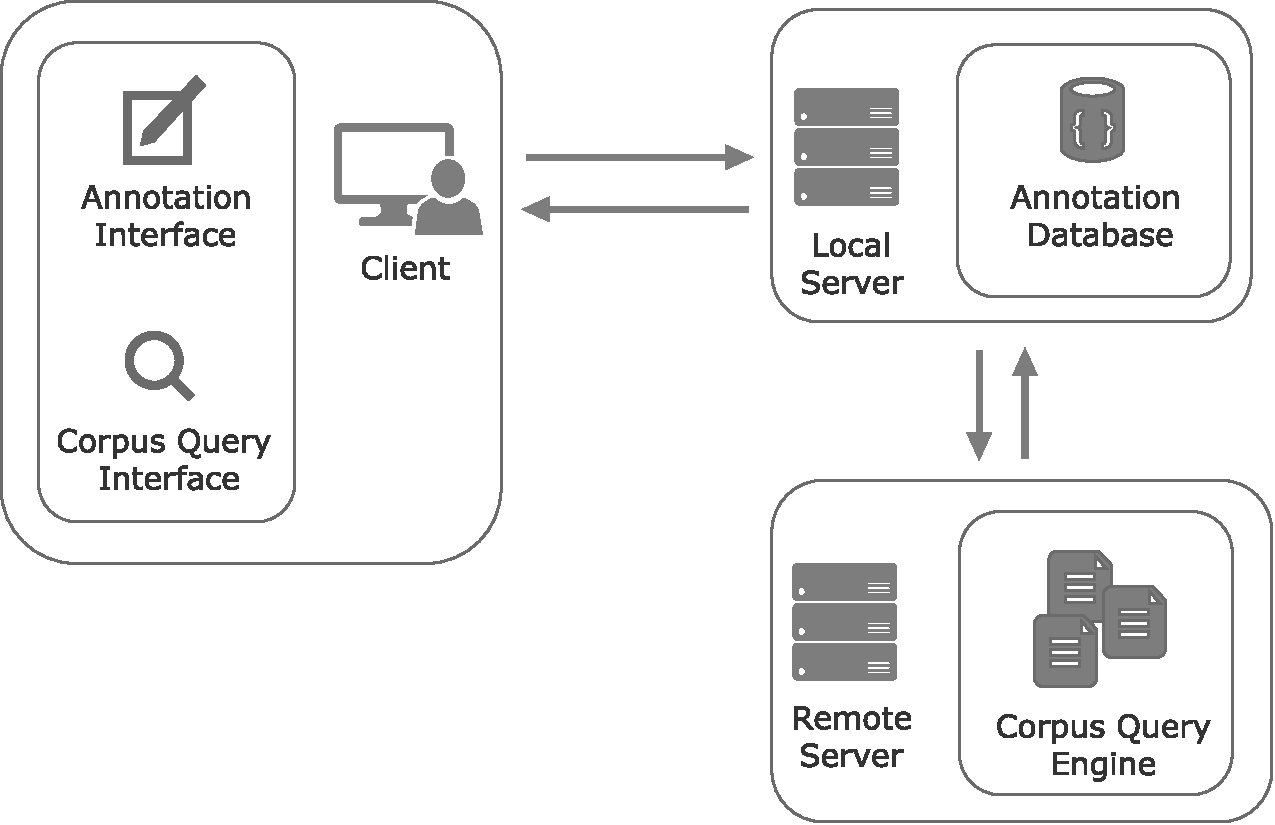
\includegraphics[width=0.45\textwidth]{./img/app-remote.pdf}
  \caption{\label{fig:app}Client-server architecture of the app}
\end{figure}

In the following sections, we describe the three layers of our application: the query engine module
(Section \ref{subsec:conc}), the version controlled metadata storage (Section \ref{subsec:db}),
and the client interface (Section \ref{subsec:client}). Finally, in Section \ref{sec:future},
we point at future research developments that arise from our infrastructure design.

\subsection{Corpus Query Engine}\label{subsec:conc}
A concordancer or corpus query engine provides the entry point to the static layer of the
application: the corpus data. Currently, we are using the Java-based corpus retrieval engine
BlackLab\footnote{
  See \texttt{https://github.com/INL/BlackLab}.
}, which is an extension to the full-text search engine Apache Lucene and provides ample and
flexible possibilities for indexing corpus documents alongside rich metadata.
As shown in Figure \ref{fig:app}, the corpus query engine may be hosted at a separate server.
User queries are forwarded to the remote server according to a REST Application Programming
Interface (API) specified by the corpus query engine server application.
For instance, a server implementation of BlackLab is available\footnote{
  See \texttt{https://github.com/INL/BlackLab-server}. Another corpus query engine offering similar
  functionality is ANNIS3.
} allowing for client queries to be forwarded as
\begin{verbatim}
  http://server/webservice/corpus/resource?parameters
\end{verbatim}
where:

\begin{description}
\item [server/webservice] is the URL of the web service,
\item [corpus] is the corpus to be queried,
\item [resource] is the type of information to be retrieved (hits, entire documents, etc..),
\item [parameters] is a sequence of URL encoded query strings specifying a query expression,
  whether to sort the results, whether to filter the results according to metadata, etc...
\end{description}

Provided a REST API server implementation for a given corpus query engine, our application can
be easily extended\footnote{
  In the next section we will review the minimal assumptions that the annotation database make on
the structure of the corpus data.
} in order to work with that corpus query engine as the backend. This way we aim to foster 
more \textbf{reusability} in corpus software development.

\subsection{Annotation Database}\label{subsec:db}
The local server is in charge of storing and retrieving the annotation metadata. Once the corpus data
are retrieved from the corpus query engine, the local server retrieves the corresponding user
annotations and merges them with the corpus data before sending the result to the client.
Additionally, it also hosts the implementation of the centralized\footnote{
  See Section \ref{subsec:workingcopy} for the distinction between centralized and distributed
  VCS systems.
} VCS features (versioning, branching, and merging) provided by the application.

\subsubsection{Annotation Metadata Model}\label{subsec:datamodel}

Our annotation metadata model is compatible with the CQP data model \cite{Christ1999} and
it is based on simple key-value structures and pointers to the token
positions to which the metadata refers. An annotation, therefore, consists of an mapping from
an annotation key to an annotation value \textemdash e.g. for a token like ``going'', we might
have an annotation key ``aspect'' associated with an annotation value ``progressive''.
In order to match annotations with the tokens to they which refer, our model has to be provided
with a unique id for each corpus token.

Furthermore, to speed up annotation queries we also require that these ids be ordered integers
\textemdash with the order corresponding to the sequence of tokens in the corpus.
Besides token annotations, our model also covers span annotations, which match annotation
key-value pairs to span of adjacent tokens in the corpus, instead of single tokens.

%% \begin{verbatim}
%%   {
%%     "ann" : {
%%       "key" : "aspect",
%%       "value" : "progressive"
%%     },
%%     "username" : "user",
%%     "project" : "periphrastic-progressive",
%%     "span" : {
%%       "type" : "IOB",
%%       "scope" : {
%% 	"B" : 416,
%% 	"O" : 41
%%       }
%%     }
%%   }
%% \end{verbatim}

\subsubsection{Versioning, Branching and Merging}\label{subsec:dbversion}

All annotations coming into the database are assigned a version. Similarly, previous values
of an annotation key are stored in the annotation version history with metadata about the author
and time of the edit as well as the corpus query that retrieved the target token(s).
As a further layer of consistency maintenance, users are only allowed to commit their changes
to other user's annotations depending on user roles and write rights assigned by the application
during setup time \textemdash i.e. if the user does not have necessary rights the update is
considered to stay in conflict with the current project version and both the author of the
current annotation and the author of the edit have to decide on the merge operation.
%% see Section \ref{subsec:client}.

While the described work pipeline enables basic versioning capabilities, it does not exploit
the concept of working copy in order to support the flexibility of VCS features as described in
Section \ref{subsec:workingcopy}. In particular, it is desirable to allow parallel work \textemdash
circumventing the conflicts that may thereby arise \textemdash and delay merging to a later point. 
Therefore, we incorporate working copies through the operation of branching in the following way.
At any point, a user may create a separate branch and start modifying annotations independently of
annotation activities by other researchers as well as write rights. Whenever the parallel work in
the branch is finished, a global merge operation with the original trunk can be issued.
This operation triggers a three-way merging algorithm in the local server which will
automatically incorporate non-conflicting changes and prompt users involved in conflicts for
a merge solution. As mentioned in Section \ref{subsec:hybrid}, user defined metadata is attached
to conflict resolutions to allow for better informed state restoration.

\subsection{Web-based Client}\label{subsec:client}

The last component of our application is a browser-based web interface that provides access to and
interaction with the search engine and the annotation database. It is designed to provide
multi-user interaction, keeping users informed of parallel work by other users and arising
annotation conflicts in real-time via notifications.

An essential feature of our front-end interface is that annotation work is always done within
so-called ``projects''. A project can be seen as a type of metadata underlying all annotations.
Users can create new projects to address particular research questions and manage user
roles and write rights. Given that each annotation is provided with project metadata,
annotation metadata queries can be done in a more specific way. Besides handling user write
rights and enabling more focused annotation queries, in our design projects provide the ground for a
publish-subscribe (pub/sub) notification pattern, according to which users can choose to
reduce the amount of live feedback of other users work by unsubscribing from particular projects.
Finally, projects are the target of the branching functionality described in Section
\ref{subsec:dbversion}. As a result of branching a sibling project is created to which
other users can subscribe.

Modern user interface design framework ReactJS, which uses functional reactive programming features
to ease the synchronization of application state with the backend model \textemdash for instance,
the client view of the annotation database with its current status.

Researchers working with large sequential datasets (such as text corpora) will most often find
themselves analyzing chunks in the absence of concurrent work by other peers\footnote{
  This is not to say that the analysis can be carried out outside the scope of a collaborative
  system since updates still have to be documented and brought to the attention of other users.
}, meaning that updates will result in conflicts with lower probability than in other setups.
We can take advantage of this fact in order to alleviate some aspects 

Annotation visualization is tailored to (KWIC with token and span annotations)

\section{Related Work, Limitations and Future Work}

Our implementation of an asynchronous collaborative annotation interface is still in development
and certain aspects are subject to improvement. In particular we would like to highlight the
following two points.

First, while the simplicity of our annotation data model provides an easily maintainable and
implementable abstraction, it does not, however, reflect current advances made by other researchers
with respect to corpus data modeling. For instance, authors related to the ANNIS project have
presented a generic, multi-layer, graph-based data model known as RelANNIS \cite{Krause2016} that
aims at covering an extensive set of annotation types (including sub-token, token, span and
tree annotations). Similarly, members of the CQP development team have recently released a working
paper describing the data model \textemdash known as Ziggurat \cite{Evert2015} \textemdash to be
used in a future release of the CQP engine. Similarly to RelANNIS, Ziggurat describes a multi-layer
data model anchored at the token level that allows to incorporate tree and graph annotations.
In the future, our annotation data model should be extended to be compatible with their
specifications (in particular, tree and graph structures).

Secondly, decoupling annotation application logic from the corpus query engine implies that
users cannot reflect the on-going body of annotations in their queries. This is, however, in
pair with the status of current corpus query engines which do not allow for incremental indexing of
new metadata. In the short-term, a less cumbersome solution can be implemented in terms of
on-demand and off-line incremental indexing \textemdash i.e. triggering corpus reindexing
to include the newly produced annotation metadata from the annotation database.

\section{Conclusions}\label{sec:conclusion}
In the present paper, we have discussed the necessity of specifically addressing issues arising
in a research context in which the annotation metadata created by multiple independent researchers
have to be synchronized. 
As a precondition to the design of appropriate collaborative tool, we have discussed the principles
behind RTE and VCS systems highlighting how they represent the synchronous and asynchronous
alternatives to the collaborative document editing problem. As result of our discussion
we concluded that research metadata curation in a collaborative environment may take better
advantage of the asynchronous features of versioning, branching and merging.

\section{Acknowledgments}
The first author wants to thank Chris Emmery for useful discussions on previous drafts of this work. 

%% \section{References}
% The following two commands are all you need in the
% initial runs of your .tex file to
% produce the bibliography for the citations in your paper.
\bibliographystyle{abbrv}
\bibliography{/home/enrique/Documents/texts/bib/library}
% You must have a proper ".bib" file
% and remember to run:
% latex bibtex latex latex
% to resolve all references
%
% ACM needs 'a single self-contained file'!
%

%\balancecolumns % GM June 2007
% That's all folks!
\end{document}
